\documentclass{article}
%for the accent
\usepackage[utf8]{inputenc}
%to put an image
\usepackage{graphicx}
\usepackage[french]{babel}
\usepackage[]{amsmath, amsfonts, amssymb, enumerate}
\usepackage{pdfpages} 

%all the things to make a good title
\title{PROJET GENIE LOGICIEL (SINFO015) :\\ Rapport de modélisation}
\author{\textbf{Auteurs}: \\ Adrien Fievet \\ Claire D'Haene \\ Julien Ladeuze \\ Maxime Dupuis}
\date{2022-2023}

\begin{document}

\maketitle

%to skip lines
\vspace{7\baselineskip}

\begin{minipage}{0.4\textwidth}
	\begin{flushleft}
		\large
		\textit{Titulaire}\\
		Tom \textsc{Mens}\\
		\textit{Enseignants}\\
		Sébastien \textsc{Bonte}\\
		Jeremy \textsc{Dubrulle}\\
		Pierre \textsc{Hauweele}	
	\end{flushleft}
\end{minipage}
~
\begin{minipage}{0.5\textwidth}
	\begin{flushright}
		\large
		\textit{Equipe 7}\\
		Adrien (220625) 4\\
		Claire (220323) 1\\
		Julien (220101) 10\\
		Maxime (212107) 7\\
	\end{flushright}
\end{minipage}

%insert the image
\begin{figure}
    \centering
    
\includegraphics[width = 0.3\textwidth]{images/umons.jpeg}
    \hspace{5em}
    
\includegraphics[width = 0.3\textwidth]{images/facSciences.png}
\end{figure}

%hide the number of the actual page just for the cover page
\thispagestyle{empty}


\newpage
\tableofcontents
\newpage

\subsection{Use cases diagrams}

\begin{flushleft}
Concernant les Use cases pour cette extension, j'ai dû en rajouter deux.
\end{flushleft}

\begin{flushleft}
\textbf{Comparer les données de consommations}, celui-ci va permettre à l'utilisateur comme son nom l'indique de comparer ses données, cette faculté a déjà été expliquée dans l'introduction.
\end{flushleft}

\begin{flushleft}
\textbf{Envoyer un mail}, quant à celui-ci, il spécifie que si une donnée d'un client est anormalement élevée, alors le serveur enverra un mail pour l'avertir, comme expliqué également dans l'introduction.
\end{flushleft}

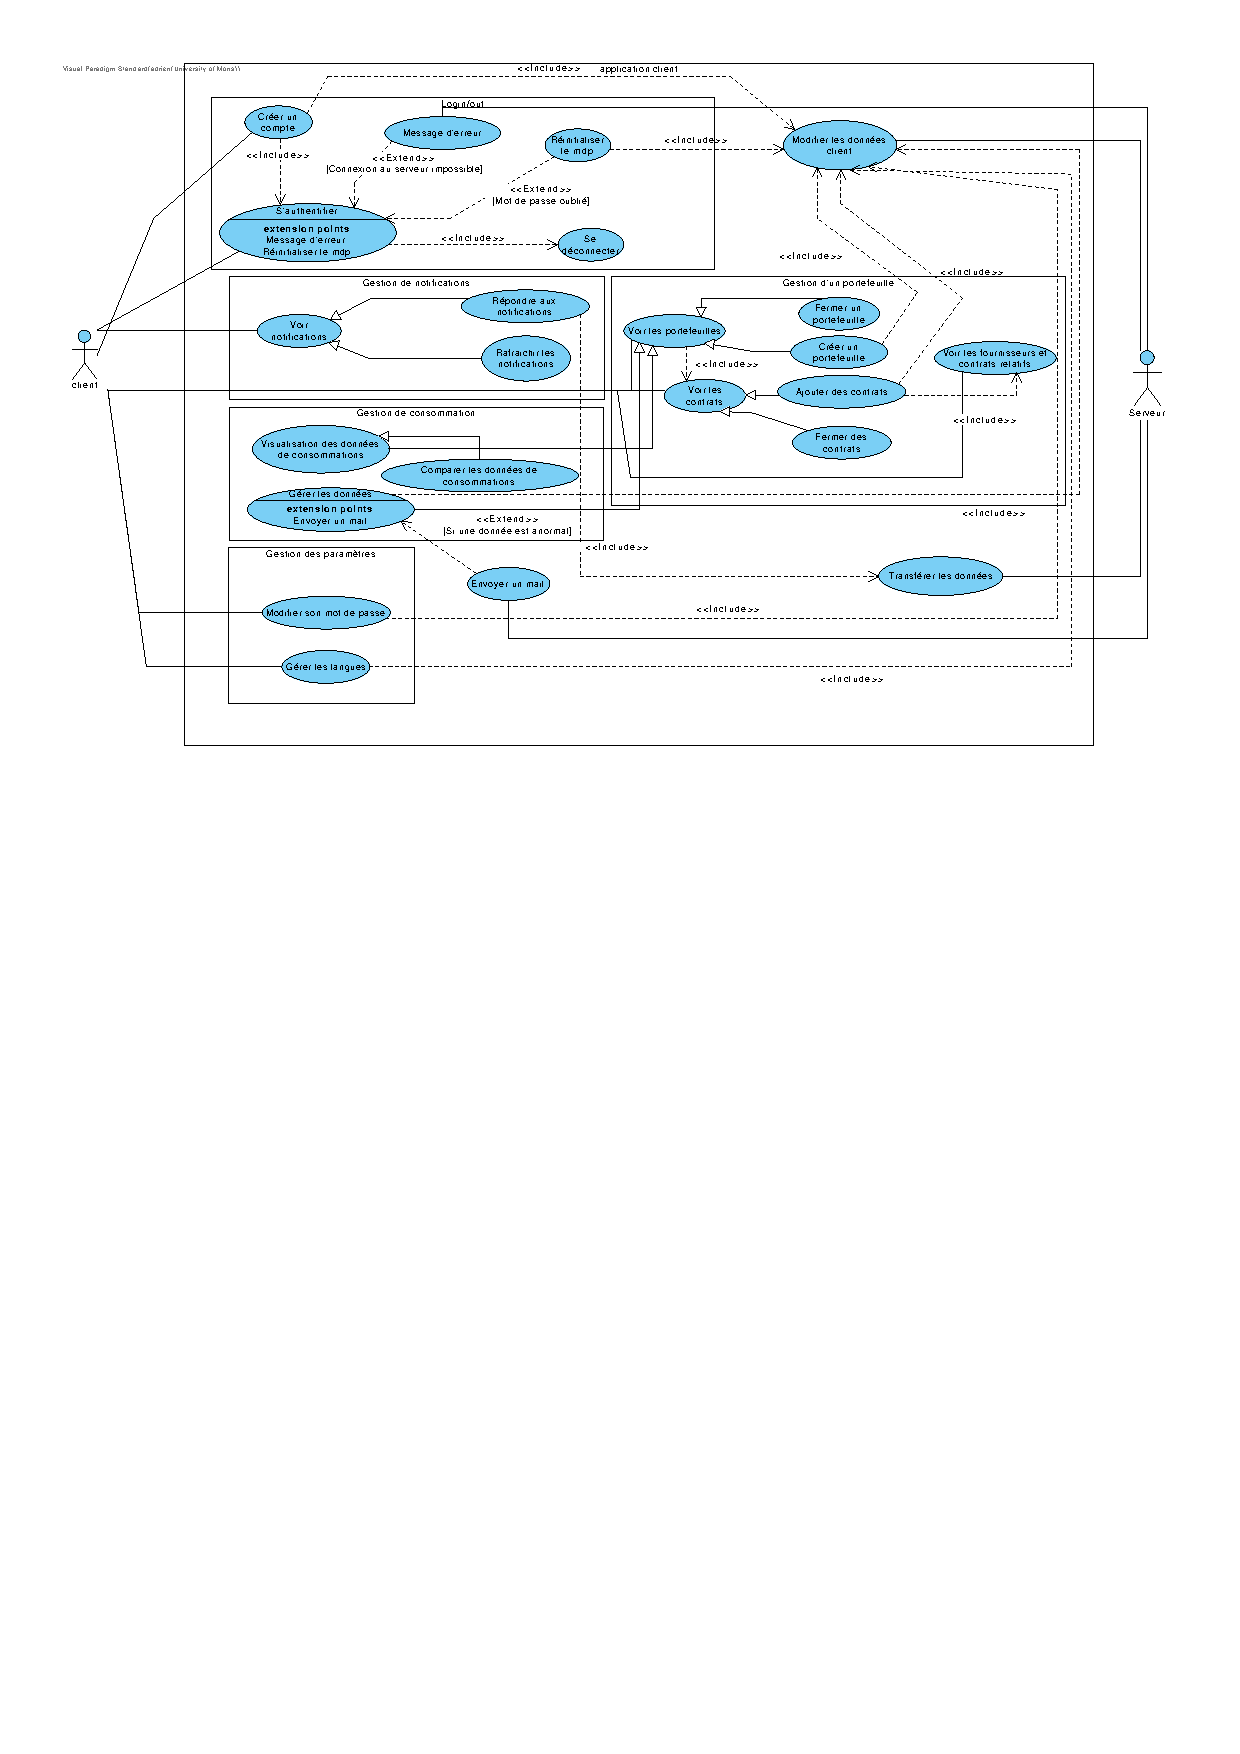
\includepdf[pages=-]{extension_adrien/use_case/img/use_case.pdf}

\subsection{Overview}

\begin{flushleft}
Au niveau de l'overview, j'ai donc ajouter un "interaction use" après la \textbf{Visualisation des données de consommation} car l'utilisateur peut décider de comparer ses données une fois qu'il est dans la visualisation s'il le souhaite.
\end{flushleft}

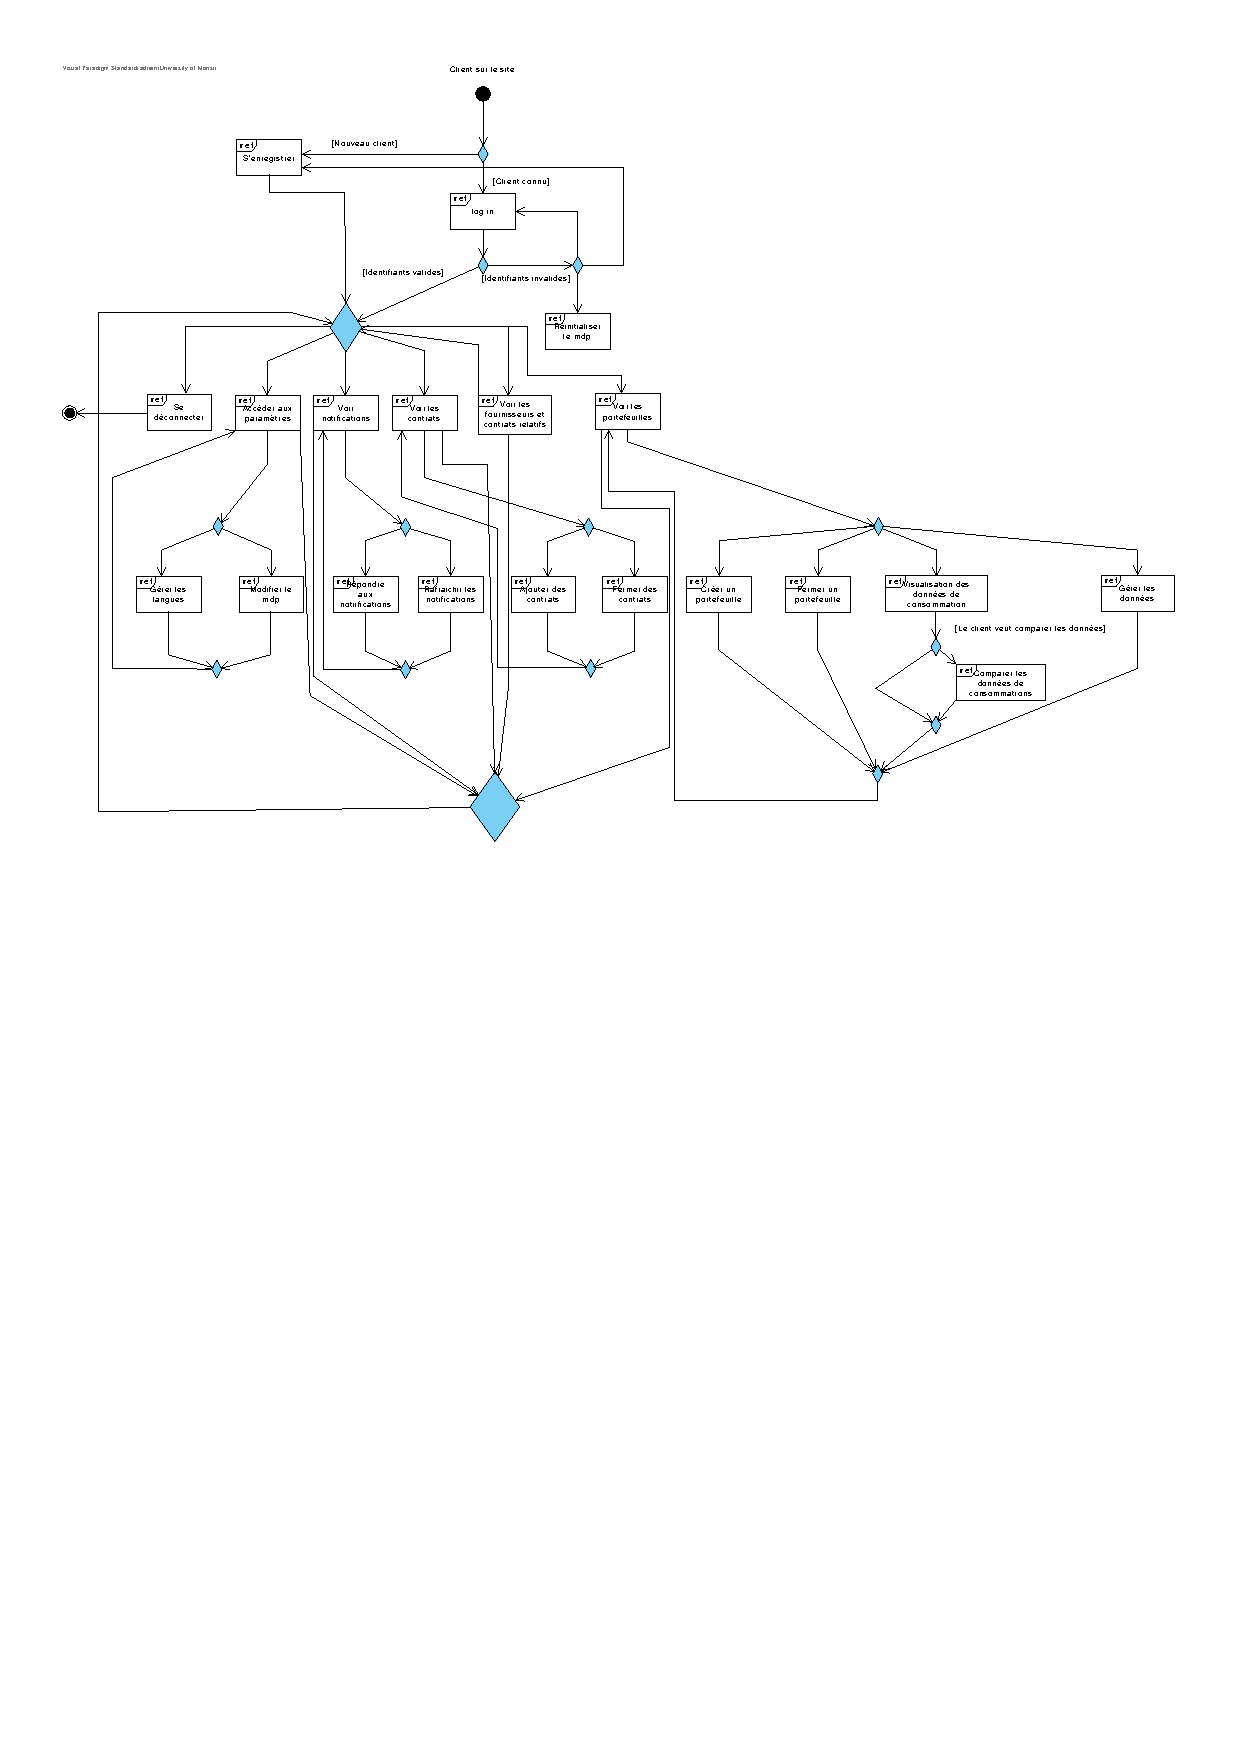
\includepdf[pages=-]{extension_adrien/overview/img/overview.pdf}

\subsection{Bdd}

\begin{flushleft}
Au niveau de la base de données, j'ai besoin dans un premier temps de stocker plus d'informations sur l'habitation des clients, c'est-à-dire dans la table \textbf{portefeuille}. Notamment le nombre de personnes habitant dans cette dernière, le type de maison, le type de chauffage et finalement s'il y a une présence de panneaux solaires.
\end{flushleft}

\begin{flushleft}
Dans un second temps, j'ai stocké les données de consommations qui serviront de comparaison. Pour cela, une nouvelle table a été crée, à savoir \textbf{consommation de simulation}. Nous devons donc y retrouver des données de consommations, un type d'énergie et une date mais il faut aussi pouvoir les distinguer en fonction des caractéristiques de la maison, c'est pourquoi nous y retrouvons également les mêmes types de données que dans la table portefeuille. C'est-à-dire le nombre d'habitants, le type de maison, le type de chauffage et s'il y a des panneaux solaires.
\end{flushleft}

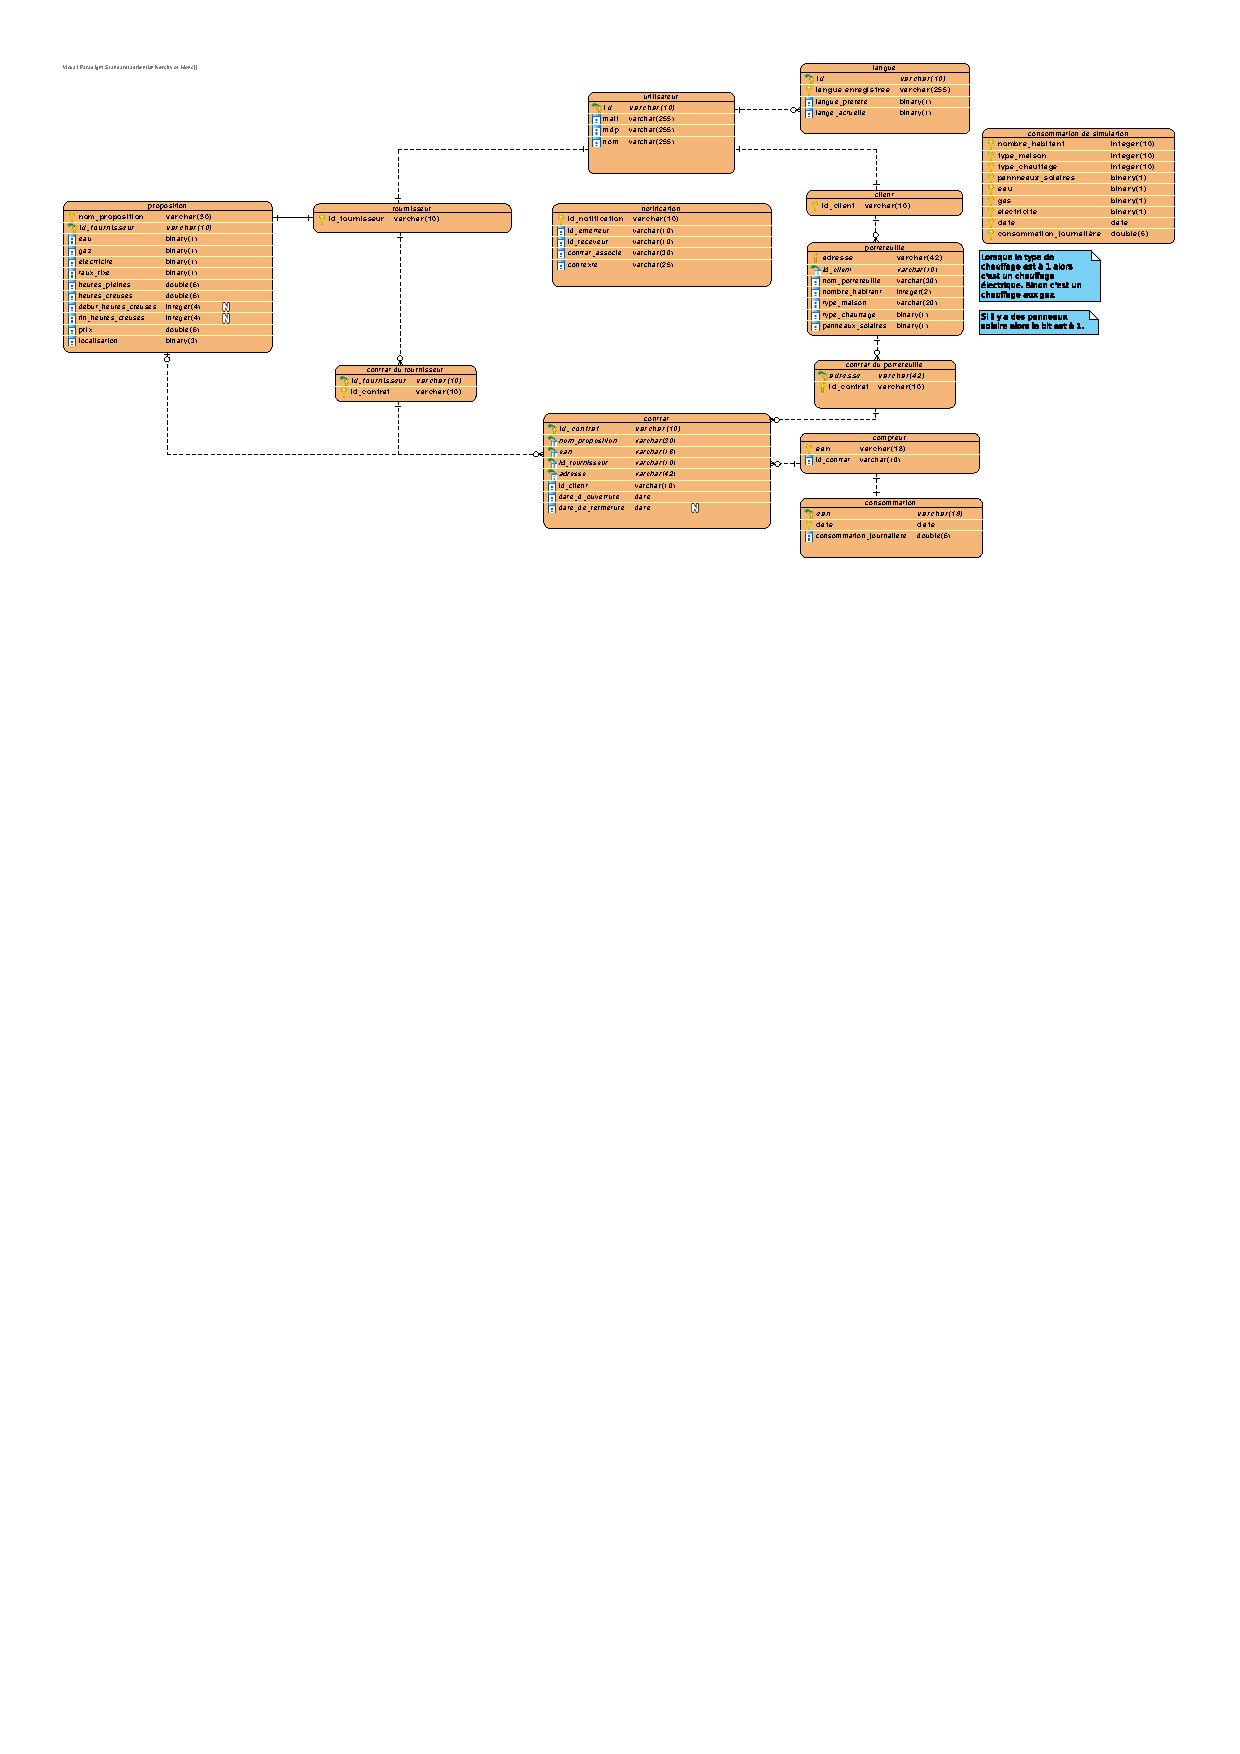
\includepdf[pages=-]{extension_adrien/Bdd/img/bdd.pdf}

\section{Diagramme des classes pour le serveur.}

\begin{flushleft}
Étant donné la taille du projet, nous avons évidemment décidé de séparer le projet en plusieurs parties. Au niveau du serveur, nous pouvons compter 3 grandes parties.
\end{flushleft}

\begin{enumerate}[-]
\item Le package api
\item Le package database
\item Le package dataObject
\end{enumerate}

\begin{flushleft}
En outre, il y a également la classe de base nommé App. Nous en reparlerons par après.
\end{flushleft}

\subsection{Le package api:}

\begin{flushleft}
Ce package contient toute la partie logique de l'ApiRest. Pour créer le serveur api nous avons décidé d'utiliser le framework Vertx, nous expliquerons notre choix dans le rapport sur l'implementation. Pour créer une ApiRest, nous avons d'abord besoin d'une classe (MyApi) qui hérite de AbstractVerticle (une classe abstraite venant du package vertx). MyApi permet de lancer le serveur à l'aide de la méthode start.
\end{flushleft}

\begin{flushleft}
Avant de la lancer, il faut d'abord configurer les routes de notre api. Notre api étant conséquente, nous avons décidé de la séparer en 4 sous-routes (parties distinctes).
\end{flushleft}

\begin{enumerate}[a)]
\item \textbf{LogApi:}\newline
Celle-ci va être utilisée pour toutes les opérations liées au login. Autrement dit, pouvoir se connecter ou se déconnecter, créer un compte et réinitialiser son mot de passe en cas d'oubli. Nous avons aussi rajouter une méthode getCode pour envoyer un code de vérification par mail lorsque l'utilisateur veut créer un compte ou pour réinitialiser son mot de passe.
\item \textbf{ClientApi:}\newline
Celle-ci va être utilisée pour toutes les requêtes liées aux clients lorsqu'ils seront connectés. Ils pourront effectuer toutes les opérations qu'ils souhaitent au niveau du portefeuille ainsi que voir tous leurs contrats et pour finir voir toutes les propositions des fournisseurs ou une en particulier. Le client pourra évidemment proposer de conclure un contrat en fonction des propositions précédemment vue.
\item \textbf{ProviderApi:}\newline
Celle-ci va être utilisée pour toutes les requêtes liées aux fournisseurs lorsqu'ils seront connectés. Ils pourront effectuer toutes les opérations qu'ils souhaitent au niveau des leurs propositions mais également voir tous les clients de l'application, tous leurs clients ou un client en particulier. Contrairement au client, il a la possibilité de supprimer une ou toutes les données de consommations liées à un contrat. De plus, tout comme le client, il pourra proposer de conclure un contrat à n'importe quelle client à partir de l'une de ces propositions.
\item \textbf{CommonApi:}\newline
Celle-ci va être utilisée pour toutes les requêtes qui sont communes aux clients et aux fournisseurs lorsqu'ils seront connectés. On y trouve les méthodes pour les langues, pour les notifications et pour les données de consommations. Il y a également une méthode pour voir un contrat en particulier et une qui permet de changer de mot de passe.
\end{enumerate}

\begin{flushleft}
Chacune de ces parties vont donc créer une sous-route grâce à la méthode getSubRouter car elles implémentent toutes l'interface Router. Et c'est donc dans la méthode start de MyApi que toutes ces sous-routes vont être rassemblées pour finalement lancer le serveur api.
\end{flushleft}

\begin{flushleft}
Notez que toutes les méthodes qui vont être appelées par l'api sont en privé car seul le serveur api peut les appeler et elles ont  le même argument (routingContext) car c'est cette variable qui contient la requête de l'utilisateur ainsi que le corps de la requête. Et c'est également par cette variable que nous pourrons répondre à l'utilisateur.
\end{flushleft}

\begin{flushleft}
Nous constatons également que ces quatre parties héritent d'une classe abstraite nommée AbstractToken. Comme son nom l'indique, elle va gérer les tokens. Autrement dit, lorsqu'un utilisateur se connecte, on va créer un token et c'est grâce à ce token qu'il pourra envoyer des requêtes aux classes clientApi, ProviderApi et CommonApi. Le token se supprimera automatiquement après un certain délai ou lorsque quand l'utilisateur se déconnectera.
\newline
Notez que si le token est expiré, l'utilisateur devra se reconnecter.
\end{flushleft}

\subsection{Le package database.}

\begin{flushleft}
Le package database contient toutes les méthodes qui vont communiquer avec la base de données. Une grande partie de celles-ci ont exactement le même nom que dans le package api puisqu’elles sont contenues dans la suite du programme. L'utilisateur envoie une requête à l'api, en fonction de la requête, la bonne méthode est appelée et appellera la méthode de database portant le même nom pour accéder aux données. Pour séparer le programme, nous avons divisé  cette partie en trois. Nous retrouvons donc une classe mère et deux classes filles.
\end{flushleft}

\begin{flushleft}
CommonDB est la classe mère de ce package, elle reprend toutes les méthodes communes aux clients et aux fournisseurs comme son nom l'indique. Outre les méthodes de l'api, nous retrouvons également les méthodes createNotification, deleteNotification et createContract car elles devront être appelées à la suite d'une requête et non directement. Nous avons aussi décidé d'ajouter les méthodes createId, getDataOfTable et deleteDataOfTable car ce sont des actions qui seront souvent utilisées et que nous pouvons donc généraliser.
\end{flushleft}

\begin{flushleft}
ClientDB et ProviderDB sont les deux classes enfants, elles s'occupent respectivement du côté client et du côté fournisseur comme leurs noms l'indiquent. Elles héritent de la classe CommonDB pour avoir accès à certaines méthodes comme par exemple createId, getDataOfTable et deleteDataOfTable. Notez qu'au niveau du client nous avons rajouté une méthode walletIsEmpty qui permet de savoir si un portefeuille du client est vide.
\end{flushleft}

\subsection{Le package dataObject.}

\begin{flushleft}
Le package dataObject contient toutes les classes représentant un objet, c'est-à-dire:
\end{flushleft}

\begin{enumerate}[-]
\item Les portefeuilles.
\item Les contrats.
\item Les clients (du point de vue des fournisseurs).
\item Les propositions (que les fournisseurs ont créées).
\item Les notifications.
\end{enumerate}

\begin{flushleft}
Notez également que nous avons rajouter une classe TypeEnergy pour énumerer tout les types d'énergies.
\end{flushleft}

\begin{flushleft}
Nous avons décidé de créer ces objets pour transférer facilement les données. En effet toutes les classes ne contiennent que des attributs avec des assesseurs à quelques exceptions près. Notez que nous aurions donc pu mettre les variables en final mais nous avons préféré laisser comme ça car dans le cas contraire nous aurions eu des constructeurs vraiment longs. Ces classes seront donc instanciées lorsque nous recevrons un objet par l'api ou quand nous prendrons des données de la base de données pour facilement les envoyer à l'utilisateur en format json.
\end{flushleft}

\begin{flushleft}
À l'exception de la classe notification, nous avons choisi de séparer chaque sorte d'objets en deux parties, une partie basique avec les informations primaires et une partie complète avec le reste des informations. Cela nous permet, lorsque l'utilisateur souhaite par exemple voir tous ces portefeuilles, d'envoyer seulement le nécessaire au lieu d'envoyer toutes les données en une fois. Ce n'est que lorsque l'utilisateur cliquera sur un portefeuille en particulier que nous enverrons toutes les données correspondant à celui-ci.
\end{flushleft}

\subsection{La classe App.}

\begin{flushleft}
La classe App est le début du programme. C'est elle qui est chargée de lancer le programme comme toutes applications java grâce à la méthode nommée "main". En effet, cette méthode va lancer l'api de la classe Myapi. Notez que nous n'avons pas directement lié ces deux classes entre elles car l'api se lance indirectement par le framework Vertx.
\end{flushleft}

\begin{flushleft}
La classe App contient également quelques méthodes statiques utilisées par les autres parties du projet. Ce sont ces méthodes qui s'occupent de la partie mail du projet, notamment "sendEmail" qui enverra une mail à un utilisateur qui souhaite créer un compte, réinitialiser son mot de passe ou bien le changer. Les autres méthodes s'occupent du "code". En effet, nous avons décidé que lorsqu'un utilisateur souhaite réaliser une des tâches précédentes, nous allons lui envoyer un code par mail avec quelques explications. Nous avons donc besoin d'une méthode pour générer le code, une pour vérifier que l'utilisateur a entré le bon code et pour finir une pour supprimer le code si l'utilisateur a mis trop de temps pour l'envoyer.
\end{flushleft}

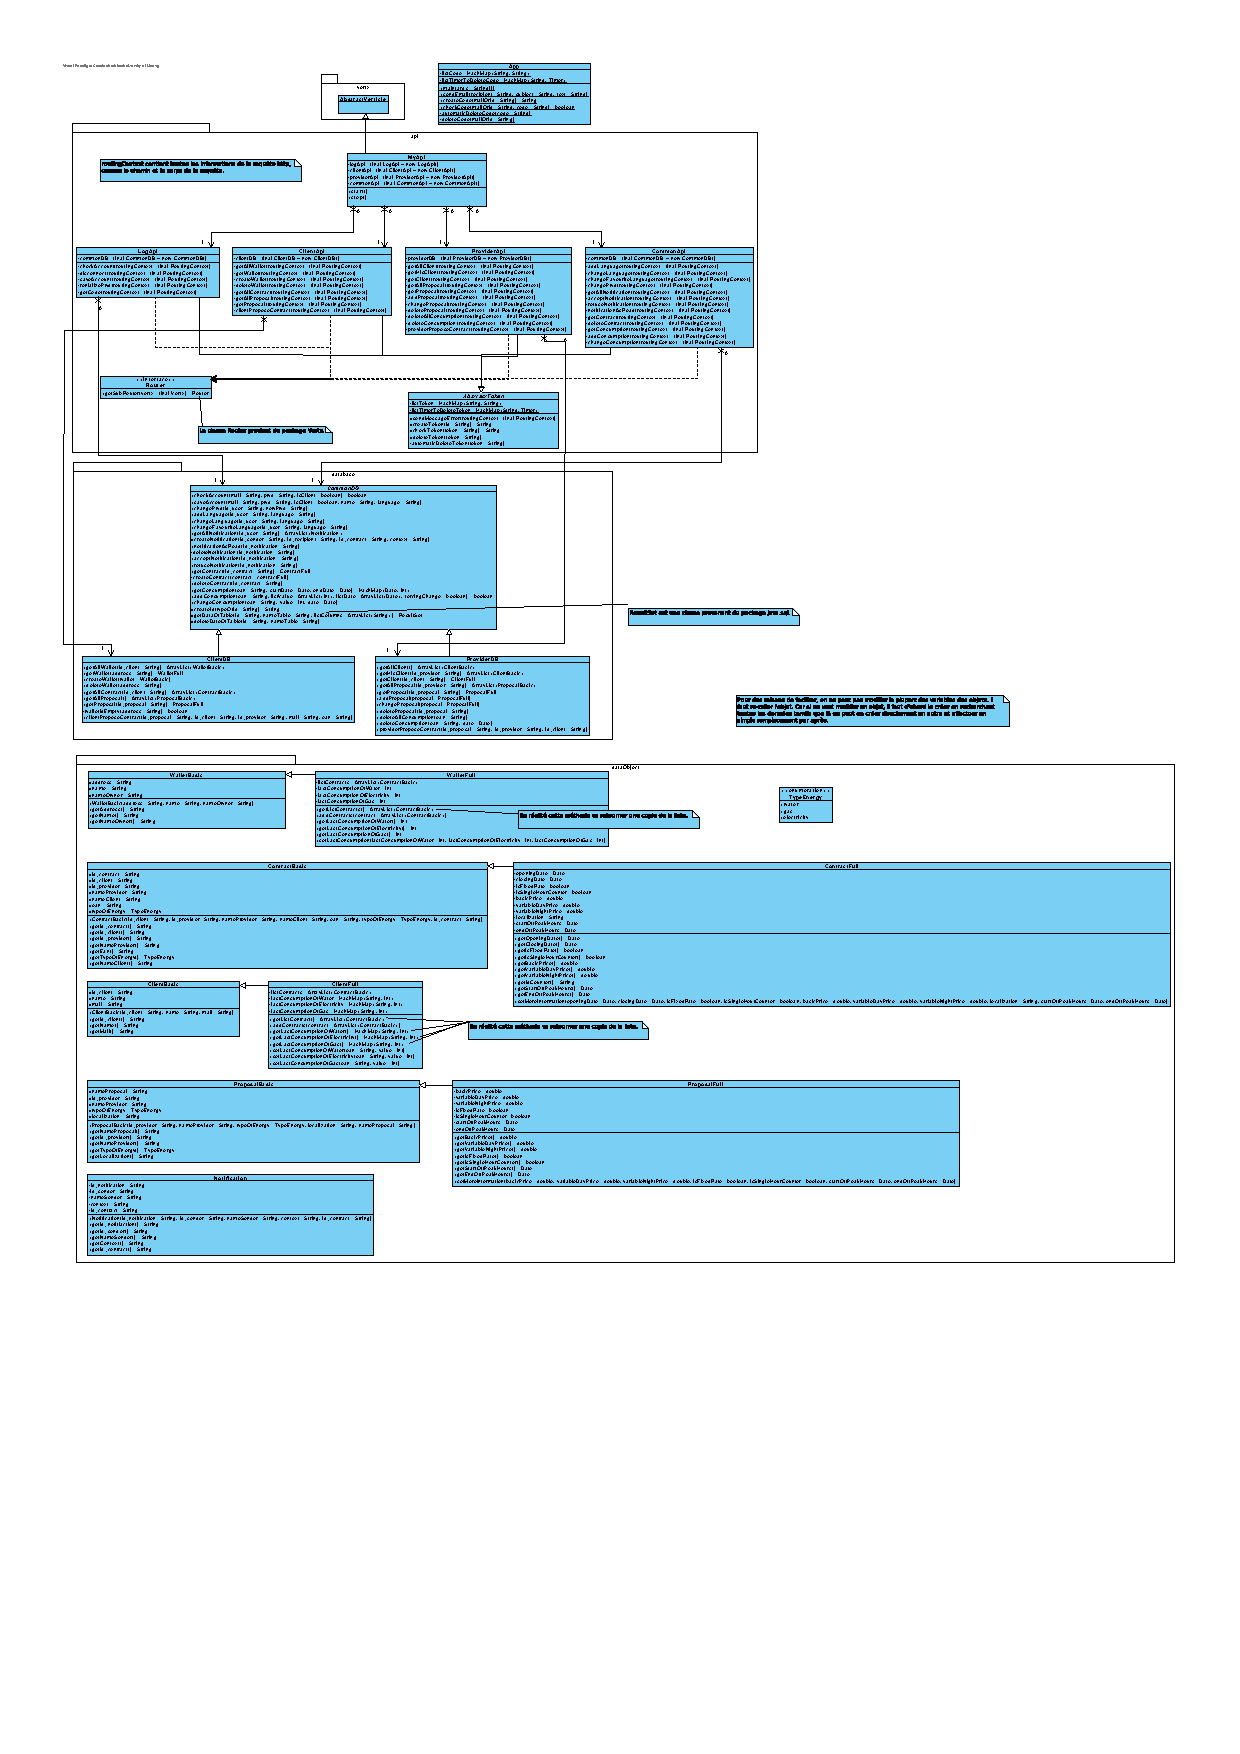
\includepdf[pages=-]{classDiagram/classDiagram.pdf}
\section{sequence}

\begin{flushleft}
Afin de compléter mon extension, j'ai introduit deux diagrammes de séquences, un premier nommé \textbf{Comparer les données de consommations} et un deuxième nommé \textbf{Gérer les données} qui est le même que celui de la base à quelques différences près.
\end{flushleft}

\begin{flushleft}
Dans le cas du premier, nous retrouvons un cas de base. c'est-à-dire que le client n'a qu'à appeler la méthode \textbf{getConsumptionOfSimulation}, le token est vérifié et si ce dernier est correct alors, dans ce cas, nous appelons \textbf{getConsumptionOfSimulation} dans la classe \textbf{ClientDB}.
\end{flushleft}

\begin{figure}[h]
\centering
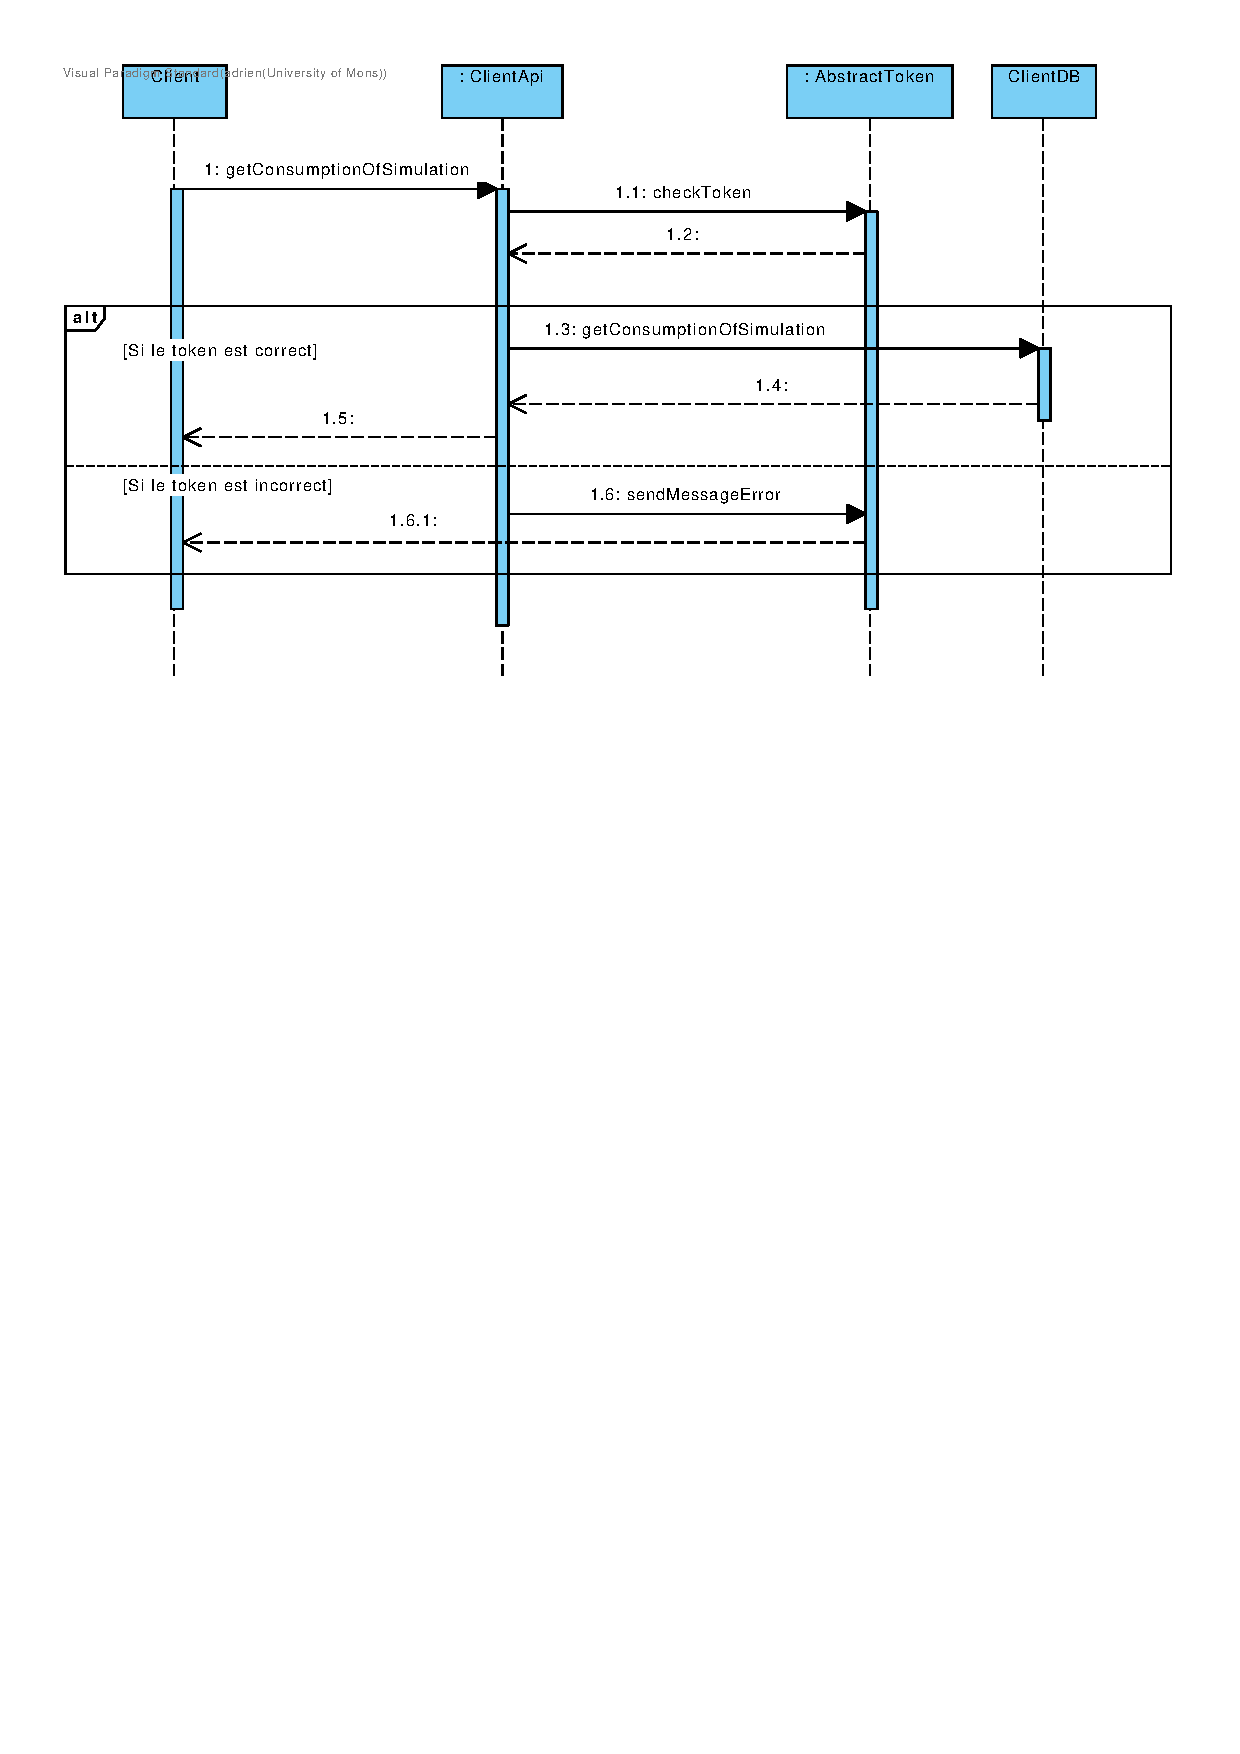
\includegraphics[width=1.3\textwidth]{extension-adrien/Sequence/img/Comparer.pdf}
\end{figure}

\begin{flushleft}
Dans le deuxième cas, que ça soit pour ajouter des données ou les changer, nous vérifions dans la classe \textbf{CommonDB} que la donnée est normale grâce à \textbf{isNormalData}. Si cette donnée est anormale, nous appelons la méthode statique \textbf{sendEmail} de la classe \textbf{App} pour envoyer un mail d'information.
\end{flushleft}

\begin{figure}[h]
\centering
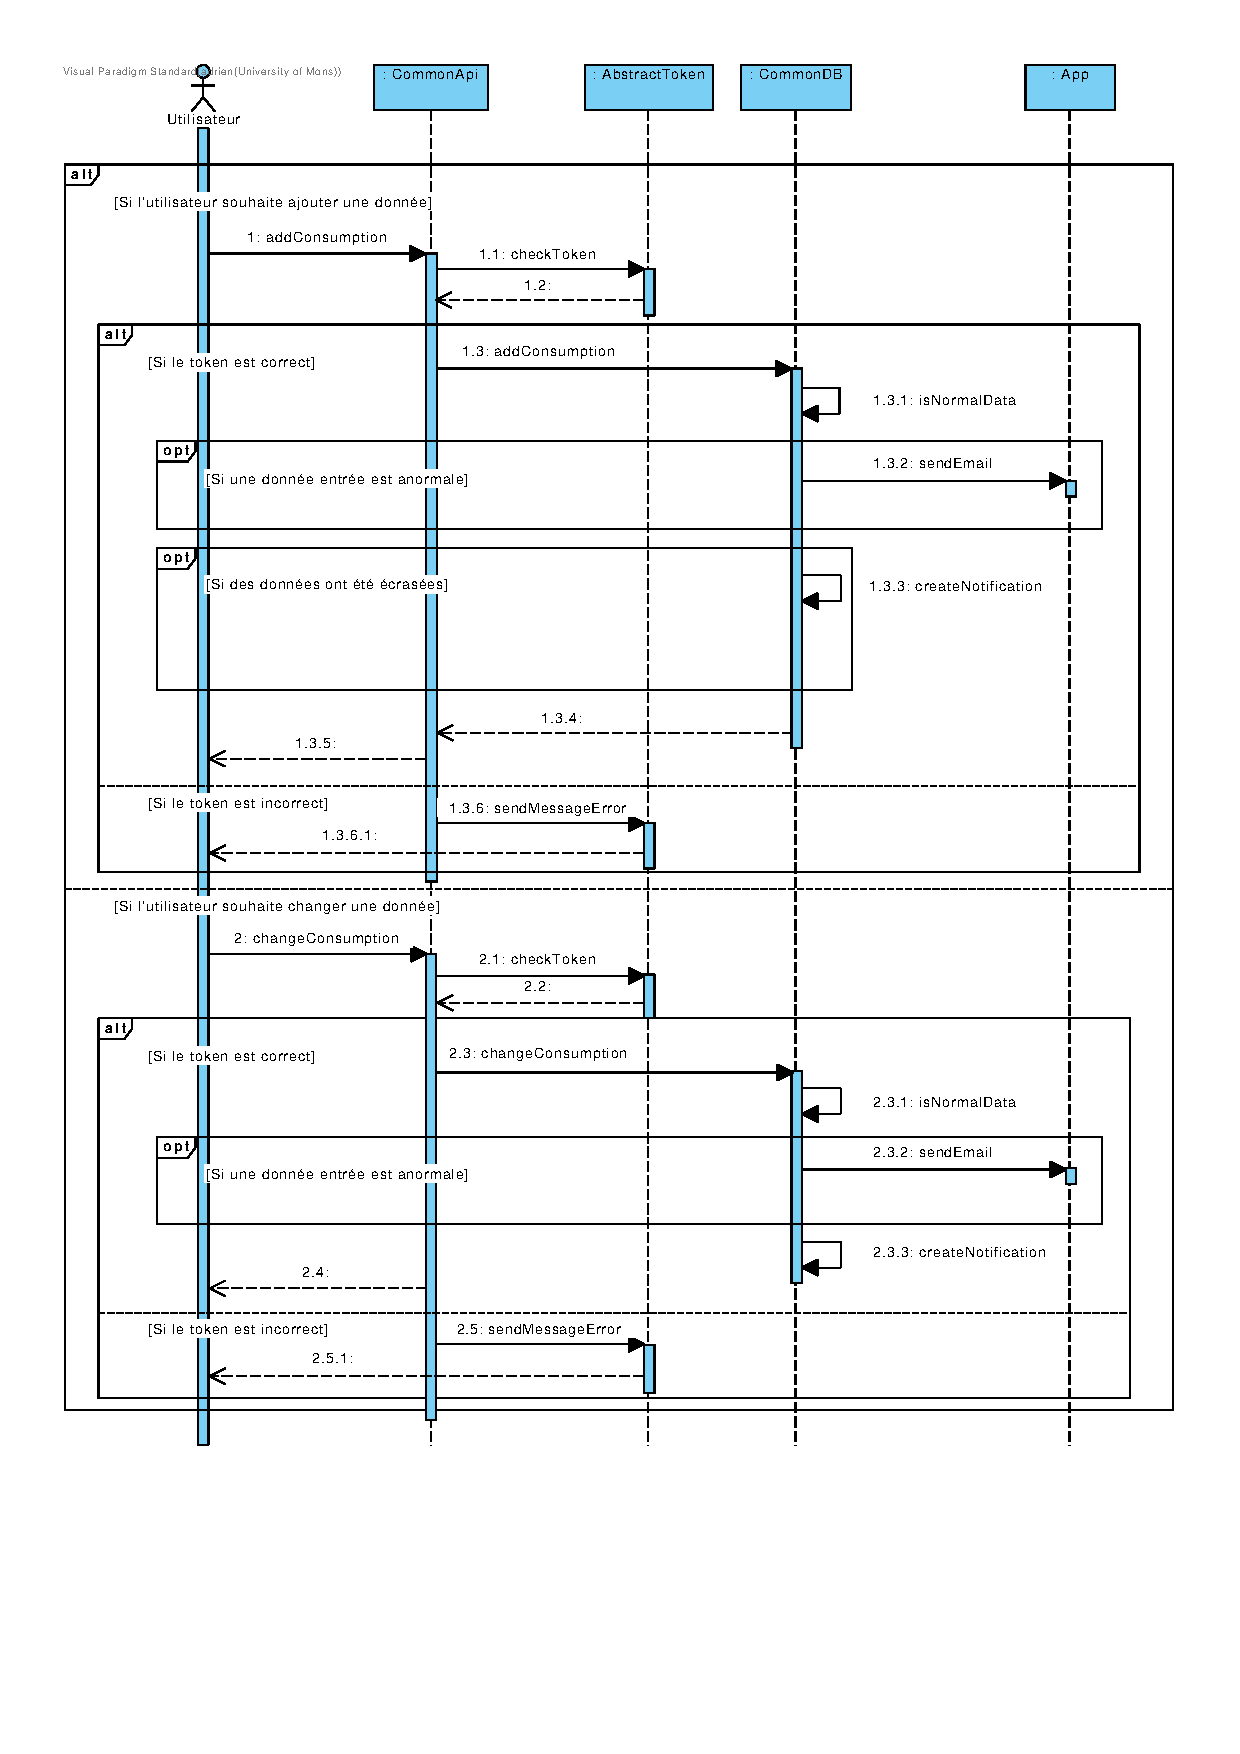
\includegraphics[width=1.3\textwidth]{extension-adrien/Sequence/img/Gerer.pdf}
\end{figure}

\subsection{Interface}

\begin{flushleft}
Pour inclure l'extension dans l'interface, j'ai dû changer 3 pages.
\end{flushleft}

\begin{enumerate}[-]
\item Add a wallet
\item Name (wallet)
\item Consumptions
\end{enumerate}

\begin{flushleft}
Suivant les explications de la base de données, le client devra entrer plus d'informations dans la fenêtre \textbf{Add a wallet} et nous pouvons également les afficher dans \textbf{Name (wallet)} vu que le client souhaite voir toutes les informations du portefeuille dans celui-ci.
\end{flushleft}

\begin{flushleft}
Dans le cas de \textbf{Consumptions}, j'ai d'abord rajouté trois boutons dans le bas de page. Ils représentent les différents modes, c'est-à-dire:
\end{flushleft}

\begin{enumerate}[-]
\item Voir sa consommation \textbf{Just see}
\item Comparer ses consommations \textbf{Compare}
\item Comparer sa consommation avec quelqu'un d'autre (simulation) \textbf{Compare with other}
\end{enumerate}

\begin{flushleft}
Finalement, j'ai placé un tableau en plus pour le cas où l'on veut comparer des données. Comme vous pouvez le voir, il y a également deux boutons au-dessus de chaque tableau qui permettent de choisir si l'on veut voir les données pures ou les statistiques.
\end{flushleft}

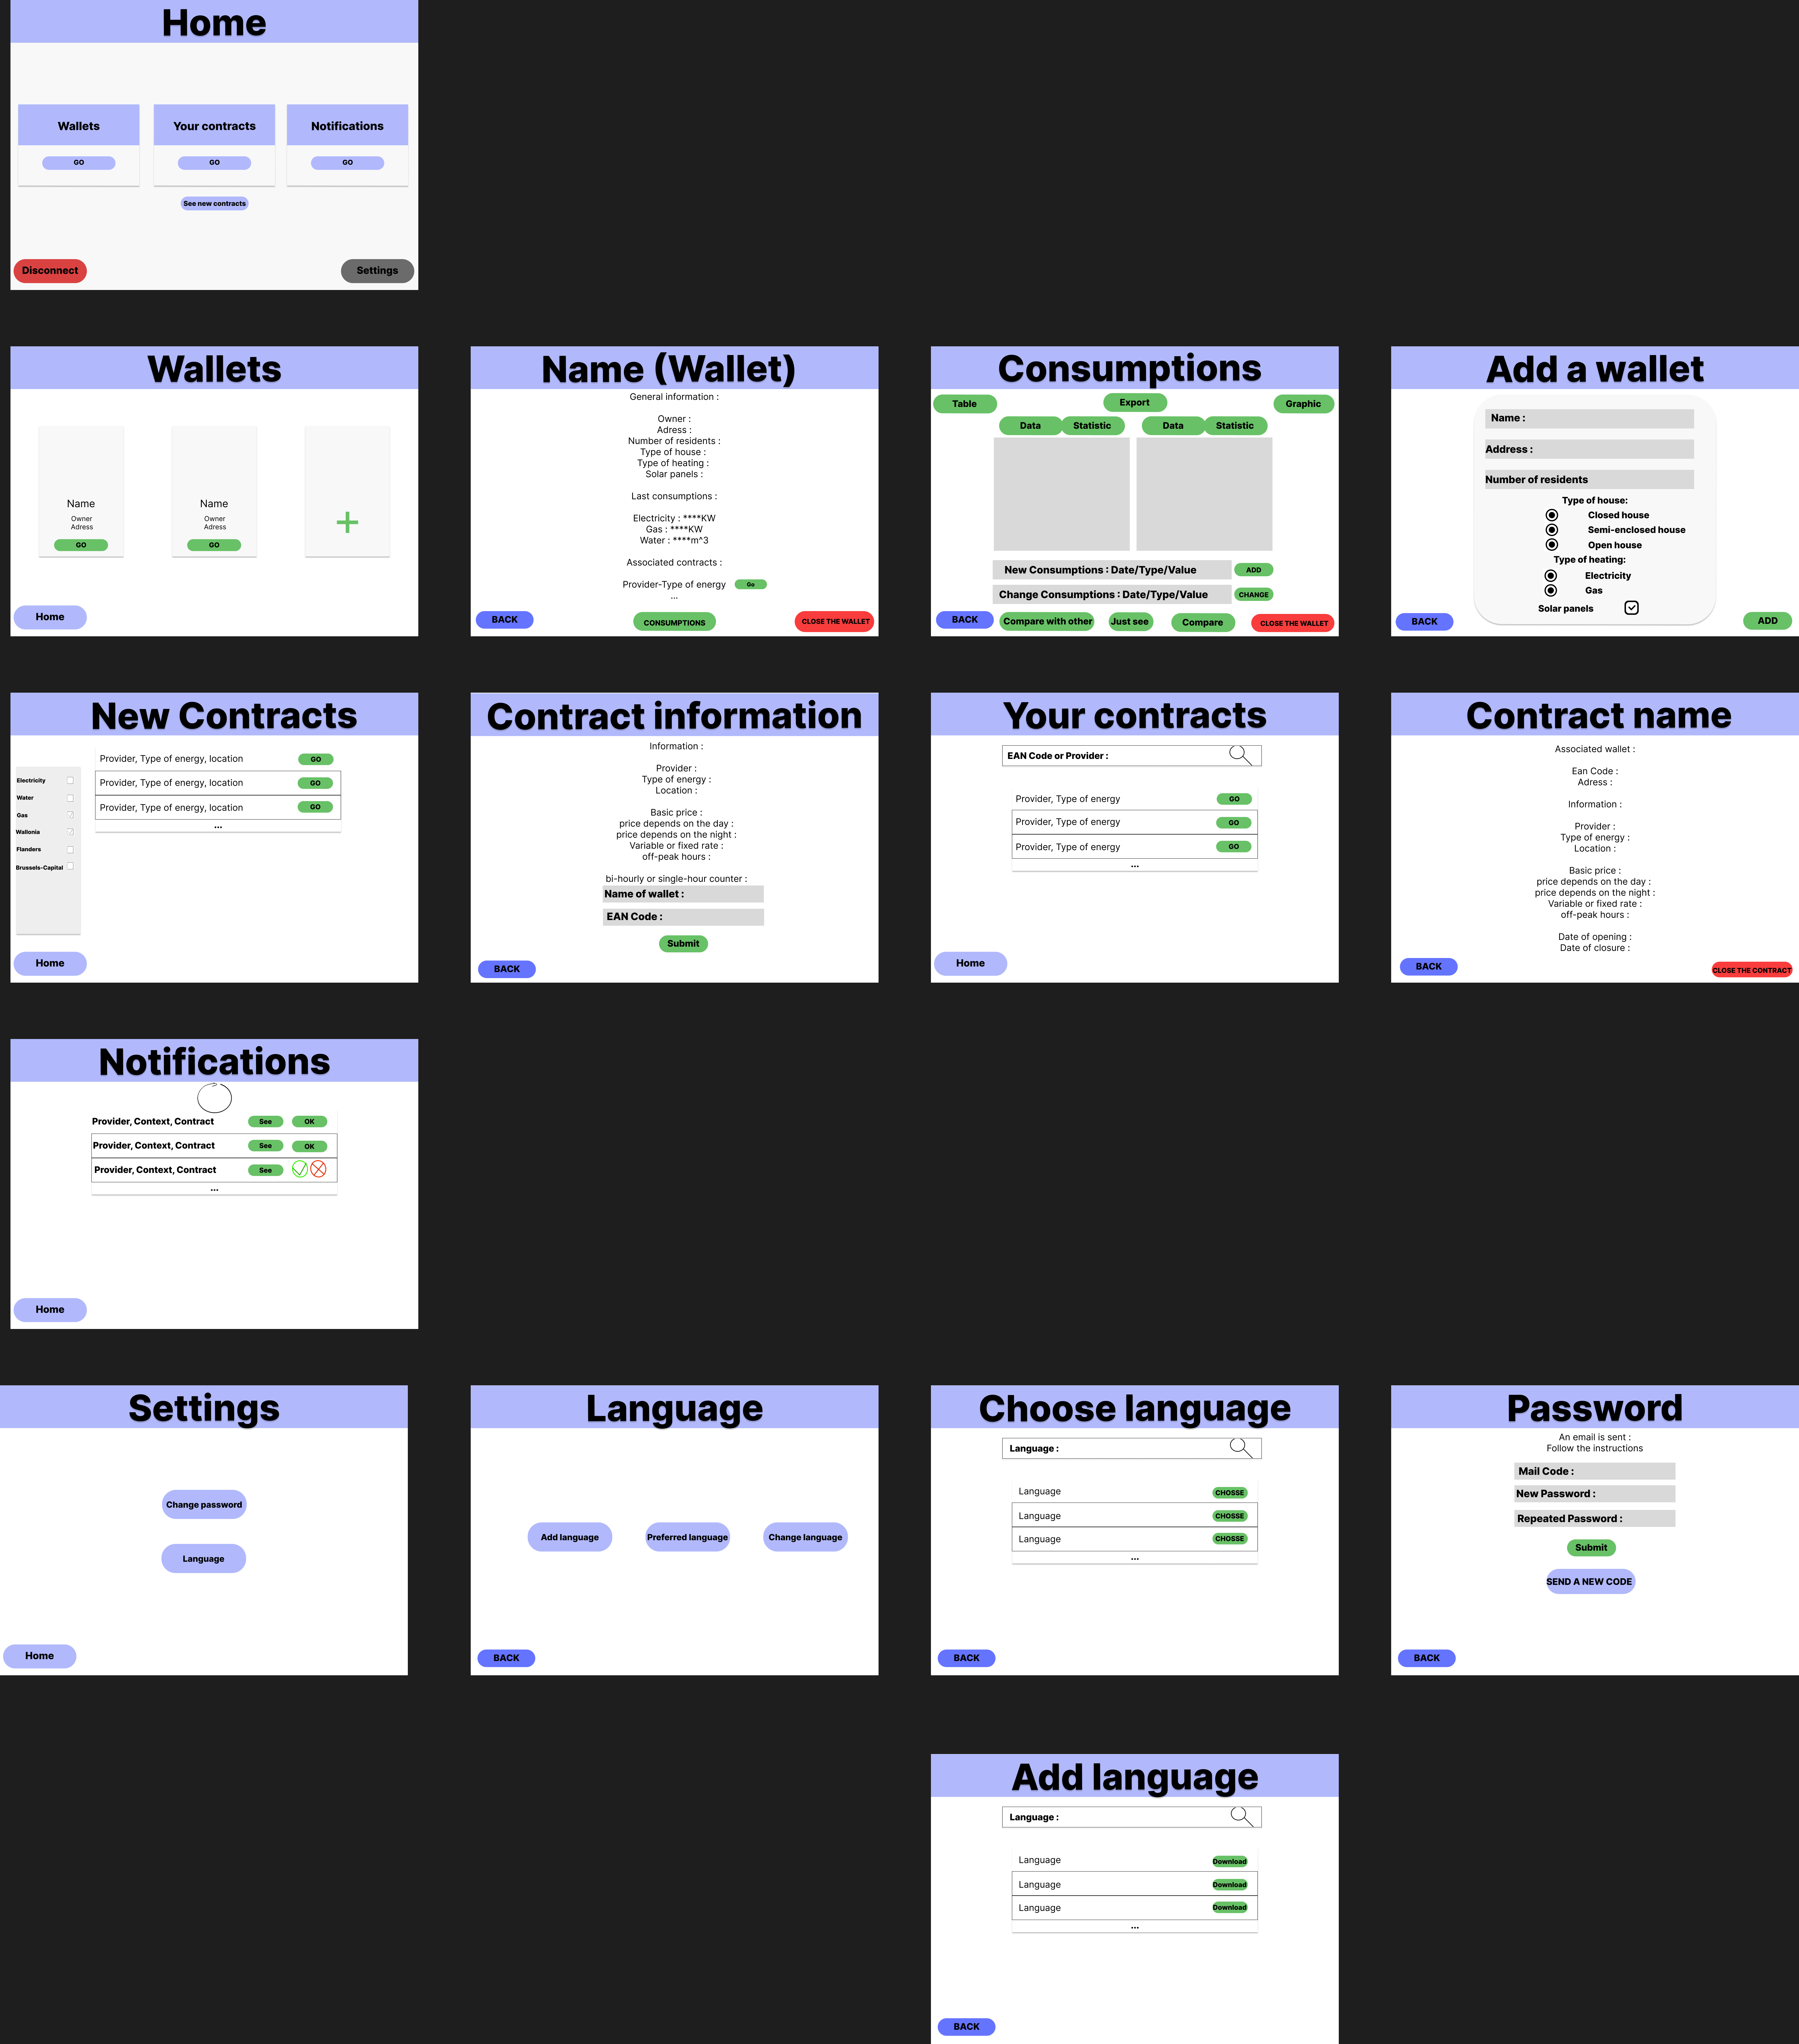
\includepdf[pages=-]{extension_adrien/Interface/img/interface.pdf}


\end{document}
